\documentclass[12pt]{article}
\usepackage[utf8]{inputenc}
\usepackage{latexsym,amsfonts,amssymb,amsthm,amsmath}
\usepackage{graphicx}
\usepackage{float}
\usepackage{caption}
\usepackage{marginnote}
\usepackage{tikz}

\setlength{\parindent}{0in}
\setlength{\oddsidemargin}{0in}
\setlength{\textwidth}{6.5in}
\setlength{\textheight}{8.8in}
\setlength{\topmargin}{0in}
\setlength{\headheight}{18pt}

\newtheorem{answer}{Answer}
\newtheorem{solution}{Solution}


\title{Weekly Homework 2}
\author{Math Gecs}
\date{December 30, 2023}

\begin{document}

\maketitle

\subsection*{Exercise 1}
A unit cube has vertices $P_1,P_2,P_3,P_4,P_1',P_2',P_3',$ and $P_4'$. Vertices $P_2$, $P_3$, and $P_4$ are adjacent to $P_1$, and for $1\le i\le 4,$ vertices $P_i$ and $P_i'$ are opposite to each other. A regular octahedron has one vertex in each of the segments $P_1P_2$, $P_1P_3$, $P_1P_4$, $P_1'P_2'$, $P_1'P_3'$, and $P_1'P_4'$. What is the octahedron's side length?
\\


 \begin{figure}[htp]
        \centering
        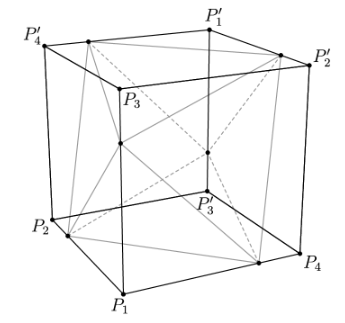
\includegraphics[width=8cm]{cube.png}
        \label{fig:assertion-cube}
     \end{figure}


Source: AMC12 (2012 - Problem 19)

\begin{answer}
$\frac{3\sqrt{2}}{4}$ \\
\end{answer}


\begin{solution}

\begin{figure}[h! tbp]
        \centering
        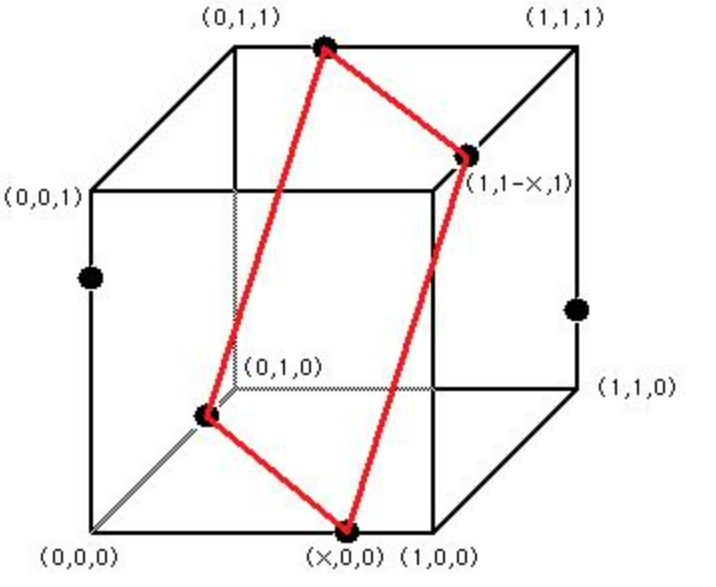
\includegraphics[width=8cm]{1.png}
        \label{fig:assertion-1}
     \end{figure}

Observe the diagram below. Each dot represents one of the six vertices of the regular octahedron. Three dots have been placed exactly x units from the $(0,0,0)$ corner of the unit cube. The other three dots have been placed exactly x units from the $(1,1,1)$ corner of the unit cube. A red square has been drawn connecting four of the dots to provide perspective regarding the shape of the octahedron. Observe that the three dots that are near $(0,0,0)$ are each $(x)(\sqrt{2}$) from each other. The same is true for the three dots that are near $(1,1,1).$ There is a unique $x$ for which the rectangle drawn in red becomes a square. This will occur when the distance from $(x,0,0)$ to $(1,1-x, 1)$ is $(x)(\sqrt{2}$).

$\\$
Using the distance formula we find the distance between the two points to be: 

$$\sqrt{{(1-x)^2} + {(1-x)^2} + 1} = \sqrt{2x^2 - 4x +3}$$

Equating this to $(x)(\sqrt{2}$) and squaring both sides, we have the equation:

$$2{x^2} - 4x + 3 = 2{x^2}$$
$$-4x + 3 = 0$$
$$x = \frac{3} {4}$$


Since the length of each side is $(x)(\sqrt{2}$), we have a final result of $\frac{3 \sqrt{2}}{4}$. Thus, Answer is $\frac{3\sqrt{2}}{4}$. 
\end{solution}

\begin{solution}
Standard 3D geometry, no coordinates. \\ 


Let the tip of the octahedron on side $P_1P_3$ be $K_1$ and the opposite vertex be $K_2$. Our key is to examine the trapezoid $P_1K_1K_2P_3$. \\ 


Let the side length of the octahedron be $s$. Then $P_1K_1 = \frac{s}{\sqrt{2}}$ and $P_3K_2 = 1 - \frac{2}{\sqrt{2}}$. Then, we have $P_1P_3 = \sqrt{2}$. Finally, we want to find $K_1K_2$, which is just double the height of half the octahedron. We can use Pythagorean Theorem to find that height as $\sqrt{2}s$. Now, we use the Pythagorean Theorem on the trapezoid. We get

$$(\sqrt{2})^2 + (2\sqrt{2}-1)^2 = (s\sqrt{2})^2$$ $$s = \frac{3\sqrt{2}}{4}$$

\end{solution}

\begin{solution}



Let the length of $P_1A = a$, $P_1B = b$
\begin{figure}[H]
        \centering
        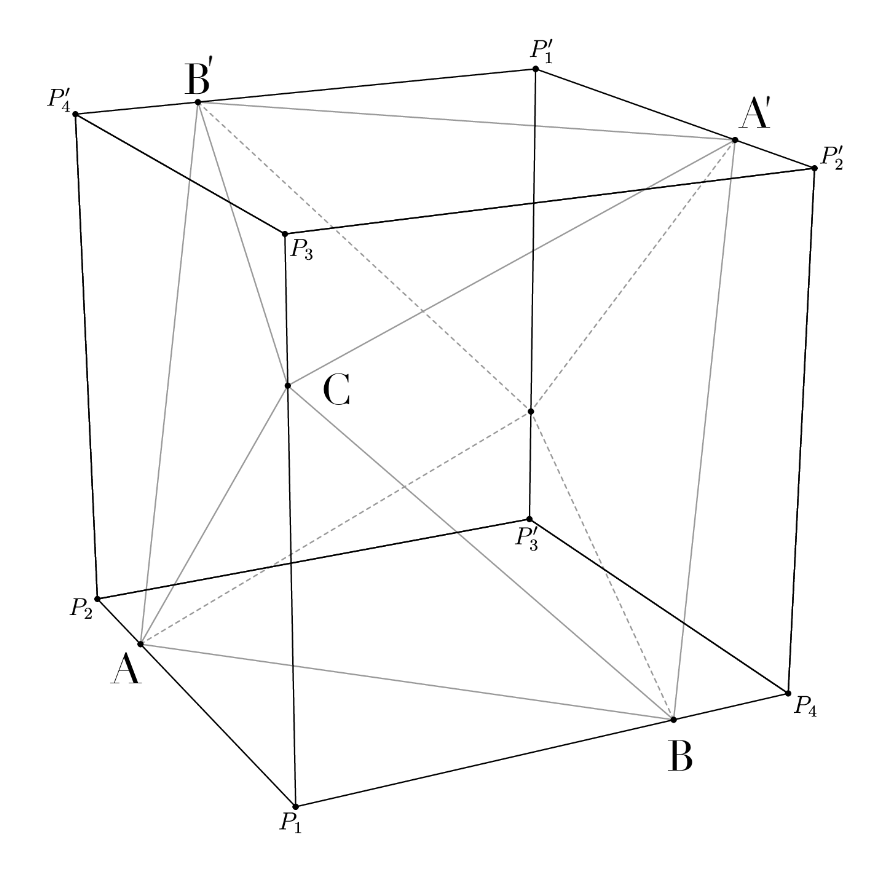
\includegraphics[width=8cm]{3.png}
        \label{fig:assertion-3}
\end{figure}
$$AB = a^2 + b^2, AB' = (1-b)^2 + (1-a)^2 + 1, AB = AB'$$
$$a^2 + b^2 = (1-b)^2 + (1-a)^2 + 1, a^2 + b^2 = 1 - 2b + b^2 + 1 - 2a + a^2 + 1, a+ b = \frac32$$
$$AC = BC, a^2 + P_1C^2 = b^2 + P_1C^2, a = b, a = \frac34$$
$$AB = \boxed{\frac{3\sqrt{2}}{4}}$$
\end{solution}

\vspace{2.3in}





\subsection*{Exercise 2}
Let $\{a_n \}_{n\ge 0}$ be a non-decreasing, unbounded sequence of non-negative integers with $a_0=0$.  Let the number of members of the sequence not exceeding $n$ be $b_n$.  Prove that for all positive integers $m$ and $n$, we have
$$ a_0 + a_1 + \dotsb + a_m + b_0 + b_1 + \dotsb + b_n \ge (m+1)(n+1) . $$
\\
Source: 1994 Balkan MO; Problem 4


\subsubsection*{Proof:}

Note that for arbitrary nonnegative integers $i,j$, the relation $j \le a_i$ is equivalent to the relation $i \ge b_{j-1}$.  It then follows that
$$ \sum_{i=0}^m a_i = \sum_{i=0}^m \sum_{j=1}^{a_i} 1 = \sum_{j=1}^{a_m} \sum_{i=b_{j-1}}^m 1 = \sum_{j=1}^{a_m} ( m+1 - b_{j-1} ) = \sum_{j=0}^{a_m-1} (m+1 - b_j ) . $$
Note that if $j \le a_m-1$, then there are at most $m$ terms of $\{ a_k\}_{k\ge 0}$ which do not exceed $j$, i.e., $b_j \le m$; it follows that every term of the last summation is positive.

Now, if $a_m \ge n+1$, then we have
$$ \begin{align*}
\sum_{i=0}^m a_i + \sum_{j=0}^n b_j &= \sum_{j=n+1}^{a_m-1}(m+1 - b_j) + \sum_{j=0}^n (m+1 - b_j + b_j) \\
&= \sum_{j=n+1}^{a_m-1}(m+1-b_j) + (n+1)(m+1) \ge (n+1)(m+1),
\end{align*} $$
as desired.  On the other hand, if $a_m < n+1$, then for all $j\ge a_m$, $b_j \ge m+1$.  It then follows that
$$ \begin{align*}
 \sum_{i=0}^m a_j + \sum_{j=0}^n b_j &= \sum_{j=0}^{a_m-1}(m+1 - b_j + b_j) + \sum_{j=a_m}^n b_j \\
&= (a_m)(m+1) + \sum_{j=a_m}^n b_j \\
&\ge (a_m)(m+1) + (n+1-a_m)(m+1) = (n+1)(m+1),
\end{align*} $$
as desired.  Therefore the problem statement is true in all cases.


\end{document}